\documentclass{beamer}
\usepackage{graphicx}
\usepackage{amsmath, amsthm, amsfonts, amssymb, mathrsfs, mathtools, caption, subcaption}
\usepackage{textcomp} % straigth apos
\usepackage{tikz}
\usepackage{verbatim}
\usepackage{listings}
\usepackage[noend]{algorithm2e}
\usepackage{float,fontawesome}
\usepackage[
  % audience=short
  audience=long
]{beameraudience}

\usetikzlibrary {arrows.meta,automata,positioning} 
\usetikzlibrary{automata}
\usetikzlibrary{shapes.geometric}

\usefonttheme{serif}

\theoremstyle{definition}

\setbeamercovered{invisible}

\setbeamertemplate{theorems}[numbered]
\setbeamertemplate{lemma}[numbered]
\newtheorem{remark}{Remark}

\usetheme{Madrid}
\useoutertheme{tree} % Alternatively: miniframes, infolines, split
\useinnertheme{circles}


\setbeamertemplate{headline}
{%
  \leavevmode%
  \begin{beamercolorbox}[wd=.5\paperwidth,ht=2.5ex,dp=1.125ex]{section in head/foot}%
    \hbox to .5\paperwidth{\hfil\insertsectionhead\hfil}
  \end{beamercolorbox}%
  \begin{beamercolorbox}[wd=.5\paperwidth,ht=2.5ex,dp=1.125ex]{subsection in head/foot}%
    \hbox to .5\paperwidth{\hfil\insertsubsectionhead\hfil}
  \end{beamercolorbox}%
}

\setbeamertemplate{section in toc}{%
  \inserttocsectionnumber.~\inserttocsection}
\setbeamercolor{section in toc}{fg=black}
\setbeamercolor{subsection in toc}{fg=structure}
\setbeamertemplate{subsection in toc}{%
  \hspace{1.2em}{\tiny\inserttocsectionnumber.\inserttocsubsectionnumber}~\small\inserttocsubsection\par}

% \setbeamertemplate{footline}{} % Remove footer
\setbeamertemplate{footline}[frame number]
\setbeamertemplate{navigation symbols}{} % Remove navigation symbols


% \setbeamertemplate{bibliography item}{\insertbiblabel.~\insertbibitem}

\definecolor{maincolor}{RGB}{78, 145, 94}

\usecolortheme[named=maincolor]{structure}

\title[End-of-studies internship]{Verification in Isabelle/HOL of Hopcroft’s algorithm for minimizing DFAs including runtime analysis}
\author[V. Trélat]{
    Vincent Trélat\\
    \small{supervised by Prof. Dr. Tobias Nipkow and Dr. Peter Lammich}
}
\institute[TUM]{Technical University of Munich\\Chair for Logic and Verification}
\date{September 2023}

\newcommand{\prompt}[1]{vtrelat@home:\raisebox{0.5ex}{\texttildelow}\$ #1}

% Outline:
% - Life in Munich
% - TUM and the Chair for Logic and Verification
%     - Teaching
%     - Research : Isabelle
% - Introduce the internship
%     - The algorithm
%     - Verification of correctness
%     - Verification of time complexity


\begin{document}

\begin{frame}
\begin{figure}
\centering
\hfill

\includegraphics[height=9mm]{../img/logoartem.png}\hfill

\includegraphics[height=9mm]{../img/logoTUM.png}\hfill
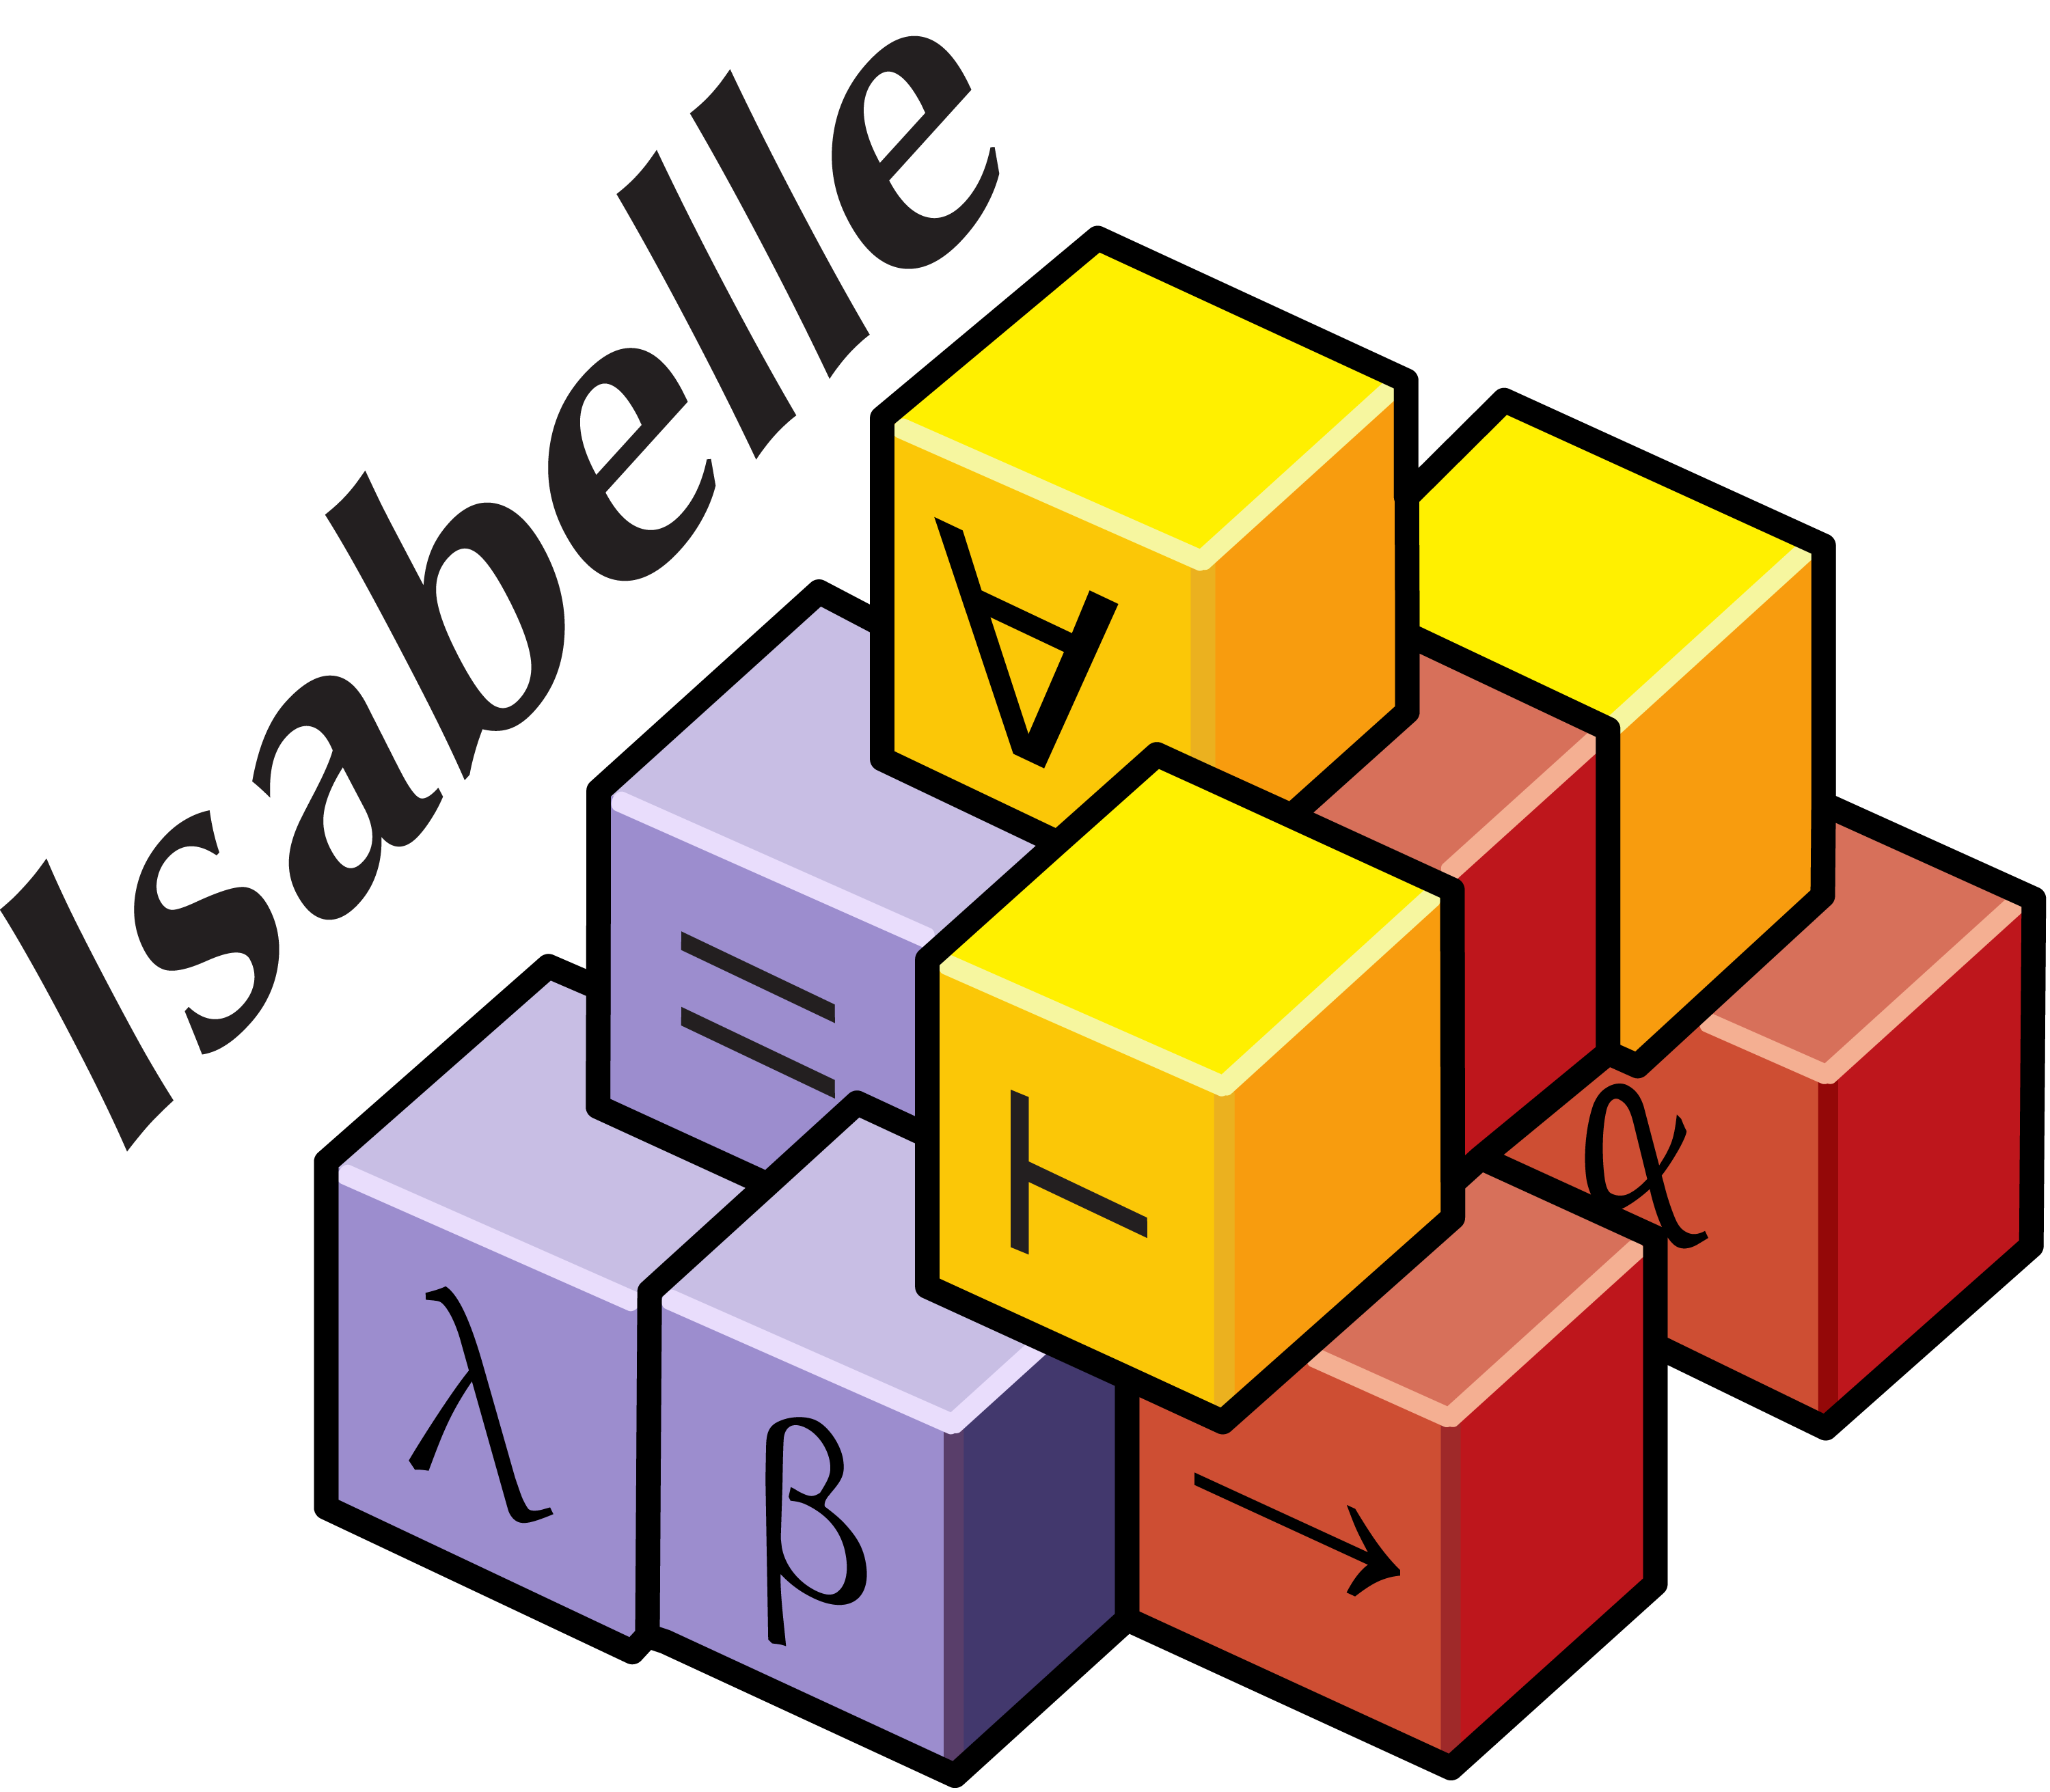
\includegraphics[height=9mm]{../img/logoisabelle.png}\hfill
\hfill
\end{figure}
\titlepage
\end{frame}

\begin{frame}
    \frametitle{Outline}
    \tableofcontents
\end{frame}

\section{Living in Munich}
\subsection{The city}

\begin{frame}
    \only<1>{
    \begin{figure}
        \centering
        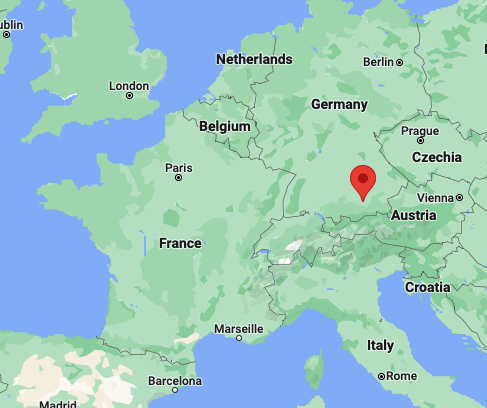
\includegraphics[width=0.7\textwidth]{img/map.png}
        \caption{Location of Munich}
    \end{figure}
    }
    \only<2>{
    \begin{figure}
        \centering
        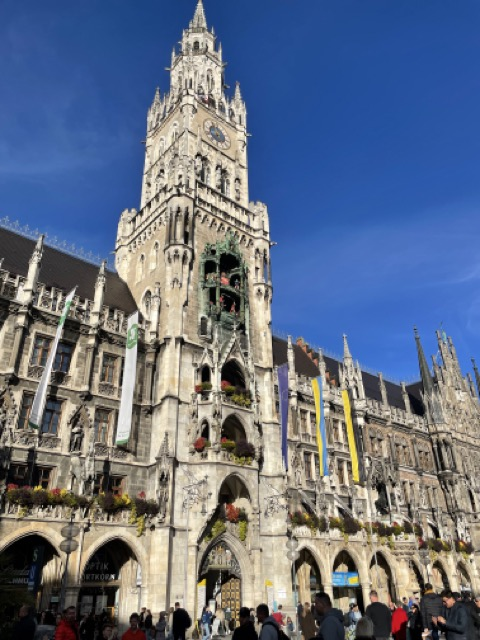
\includegraphics[height=4cm]{img/munich1.jpeg}
        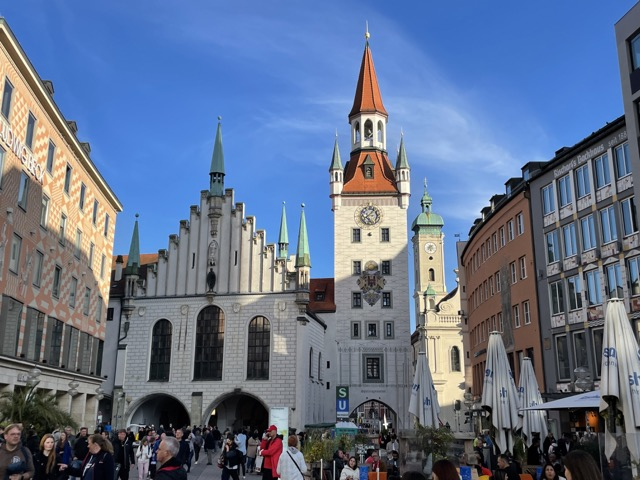
\includegraphics[height=4cm]{img/munich2.jpeg}
        \vfill
        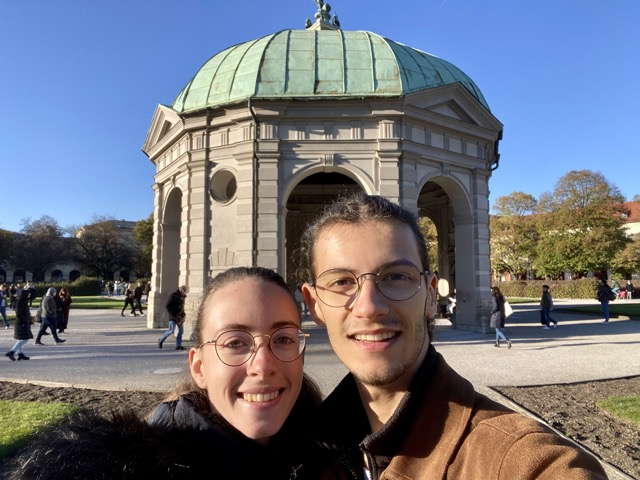
\includegraphics[height=4cm]{img/munich3.jpeg}
        \caption{Some photos of Munich}
    \end{figure}
    }
\end{frame}

\subsection{Technical University of Munich}

\begin{frame}
    \only<1>{
    \begin{figure}
        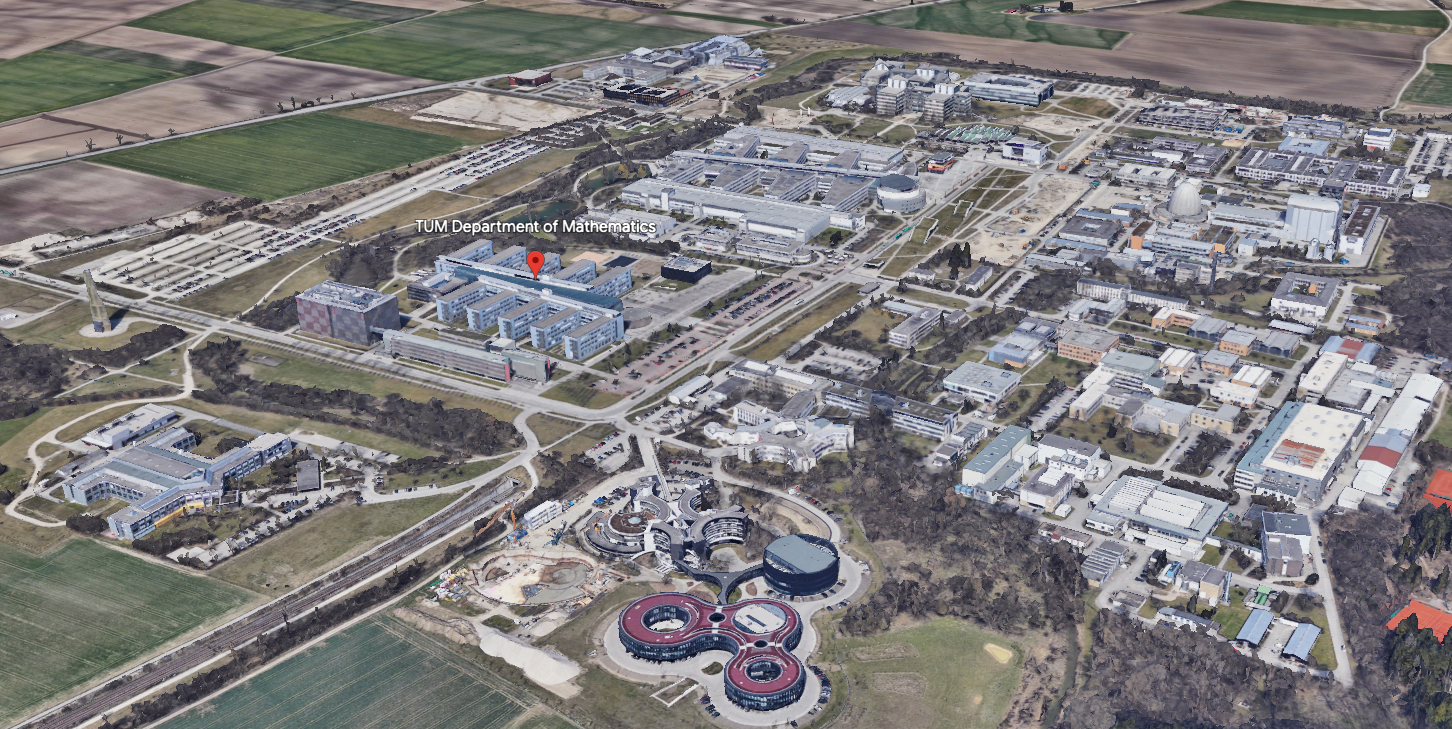
\includegraphics[width=\textwidth]{img/TUM_aerial.png}
        \caption{Technical University of Munich (TUM), Garching campus}
    \end{figure}
    }
    \only<2>{
    \begin{figure}
        \begin{subfigure}{0.3\textwidth}
            \centering
            
\includegraphics[height=1cm]{../img/logoTUM.png}\\
            \vspace*{1cm}
            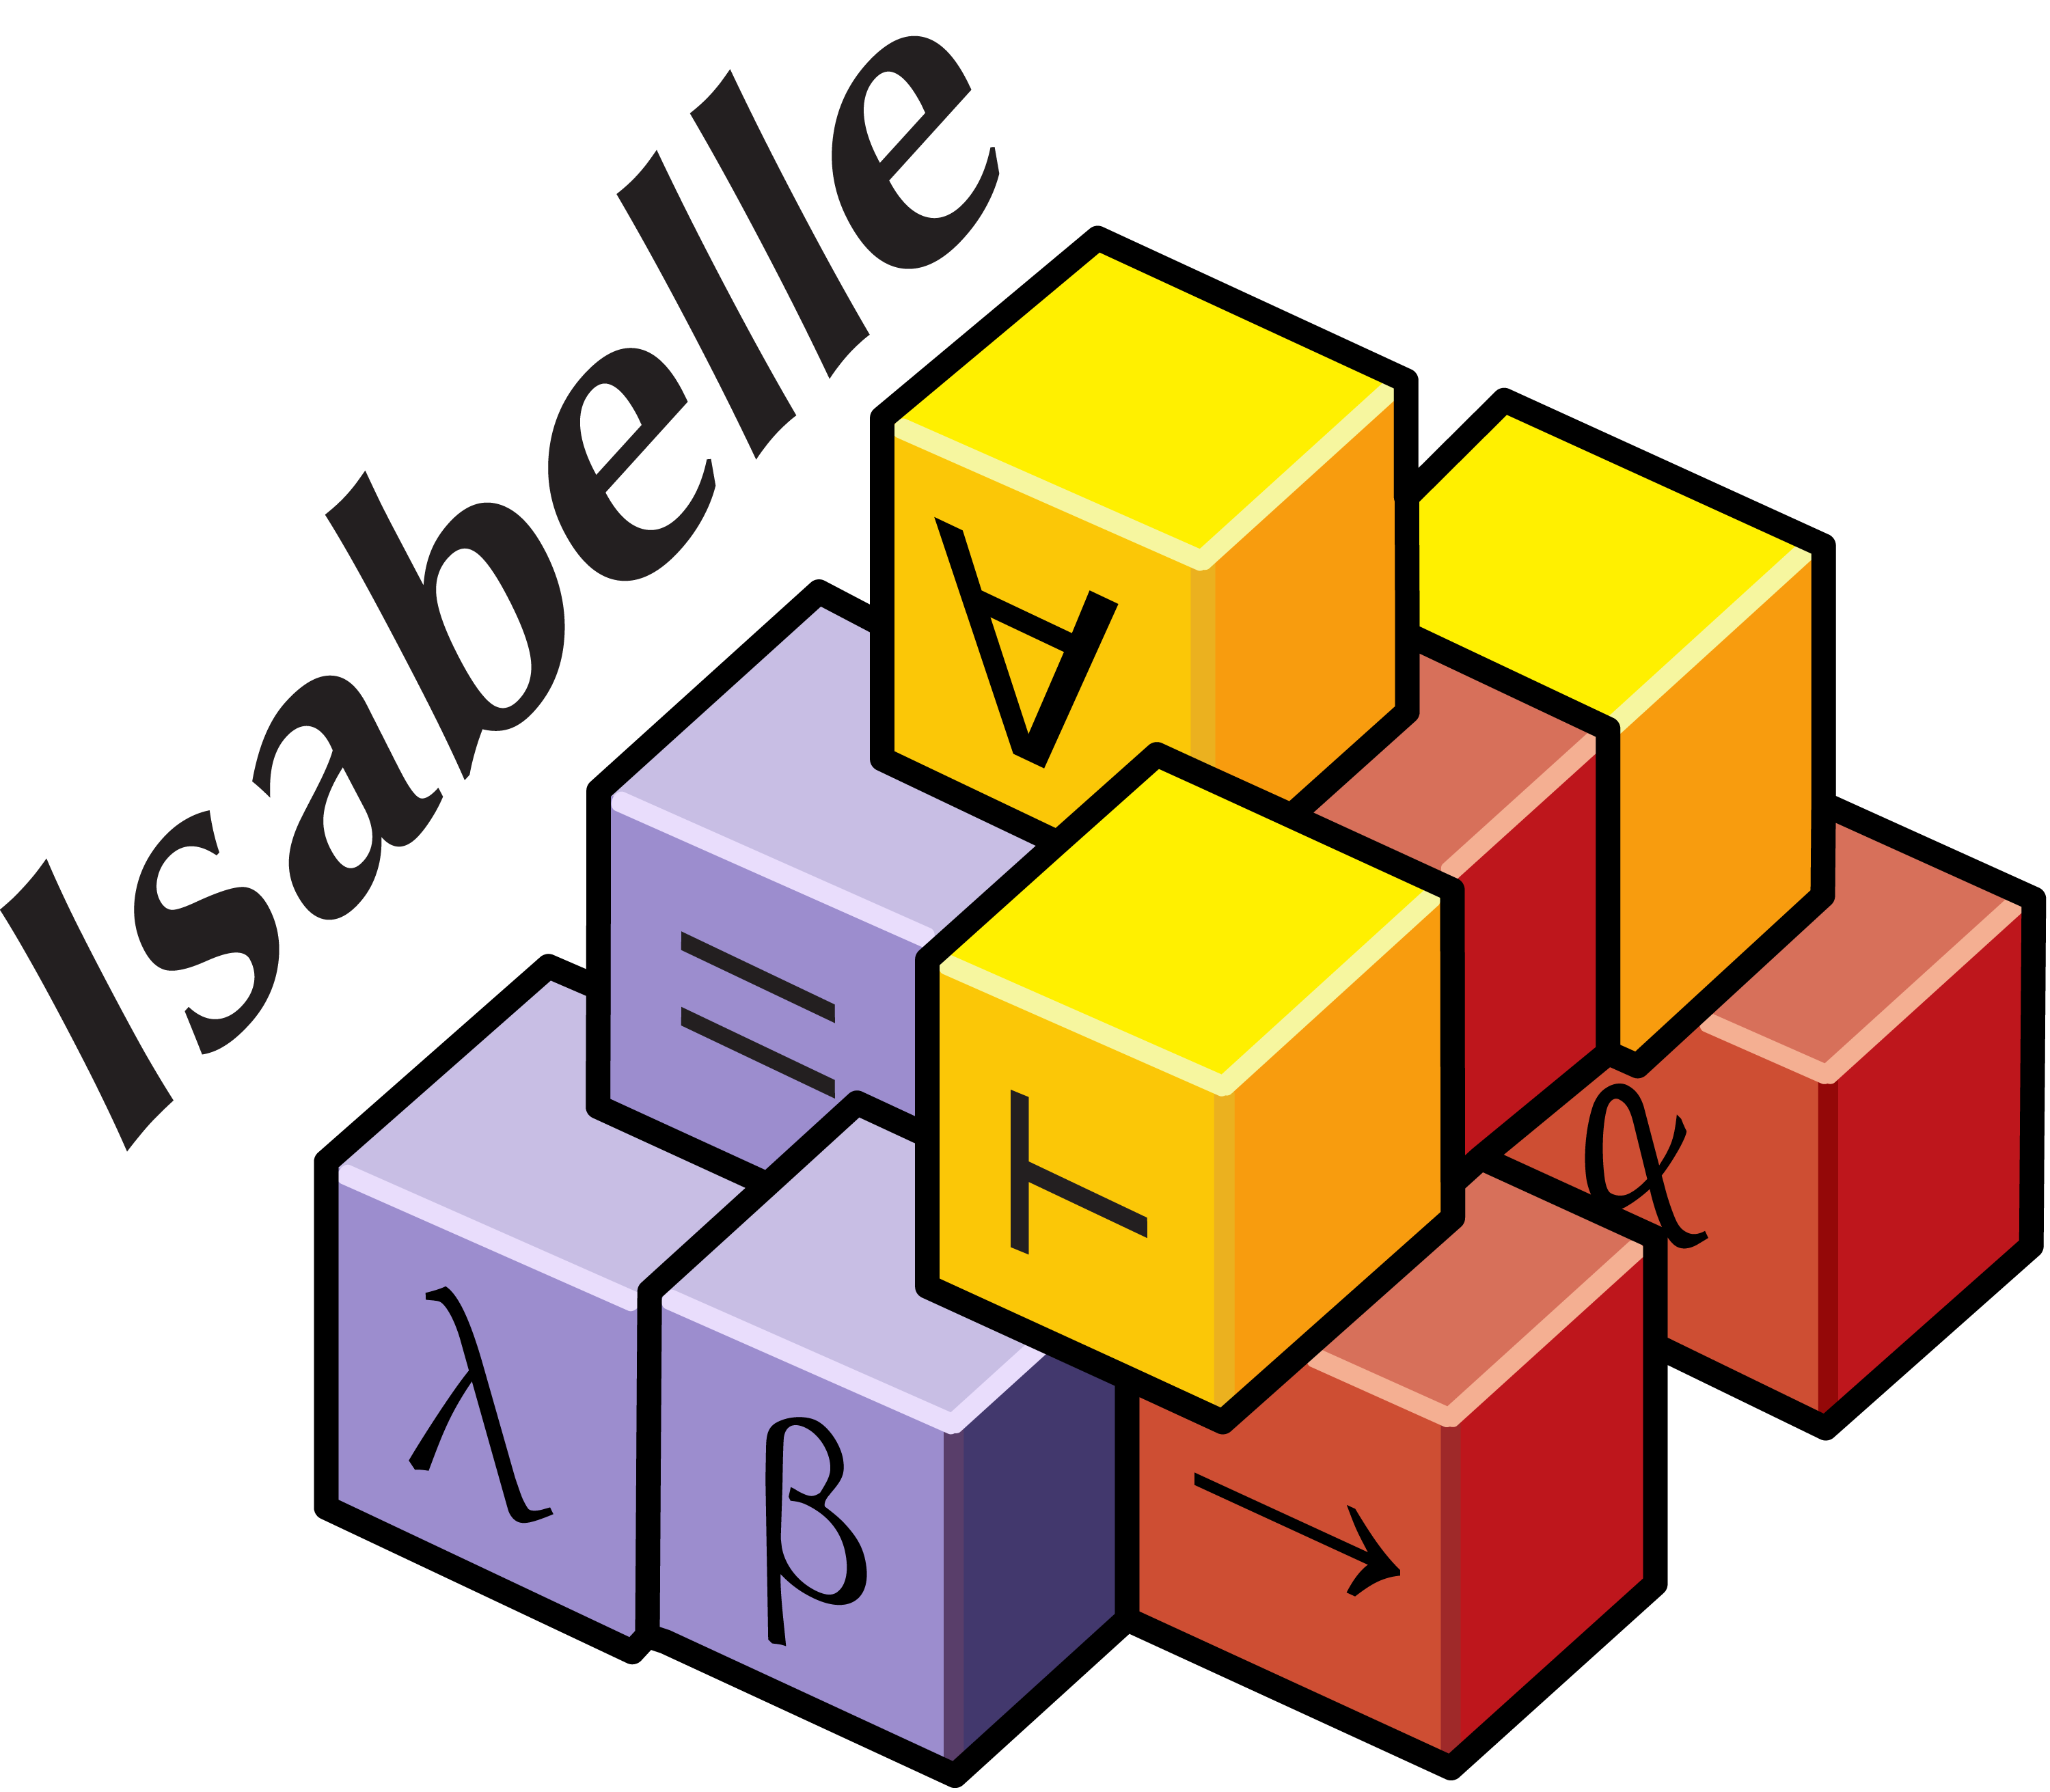
\includegraphics[height=1.5cm]{../img/logoisabelle.png}
        \end{subfigure}
        \begin{subfigure}{0.69\textwidth}
            \centering
            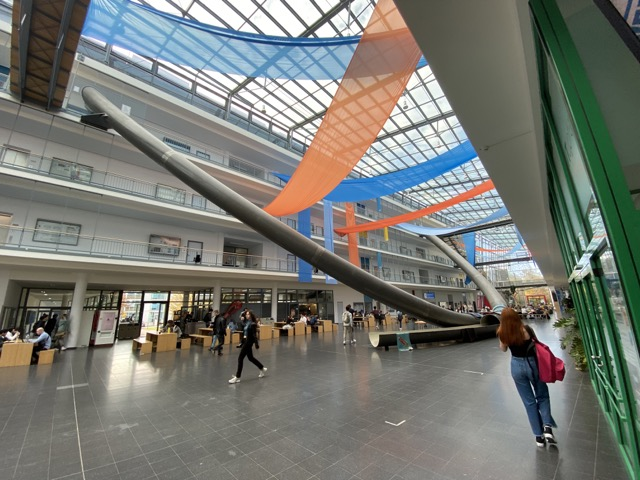
\includegraphics[height=6cm]{img/TUM.jpeg}
        \end{subfigure}
        \caption{Technical University of Munich (TUM), Garching campus}
    \end{figure}
    }
\end{frame}

\begin{frame}
\onslide<+->{
\begin{figure}
    \centering
    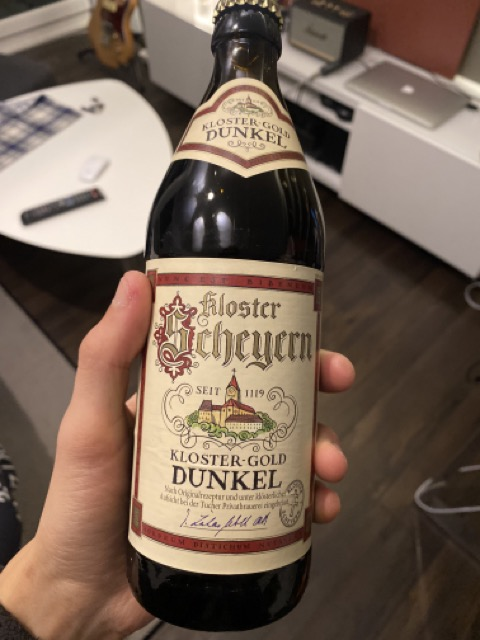
\includegraphics[height=3cm]{img/beer0.jpeg}
    \onslide<+->{
\includegraphics[height=3.2cm]{img/beer1.jpeg}}
    \onslide<+->{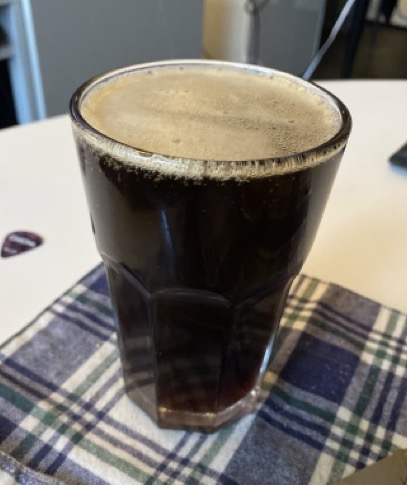
\includegraphics[height=3.2cm]{img/beer2.jpeg}}
    \onslide<+->{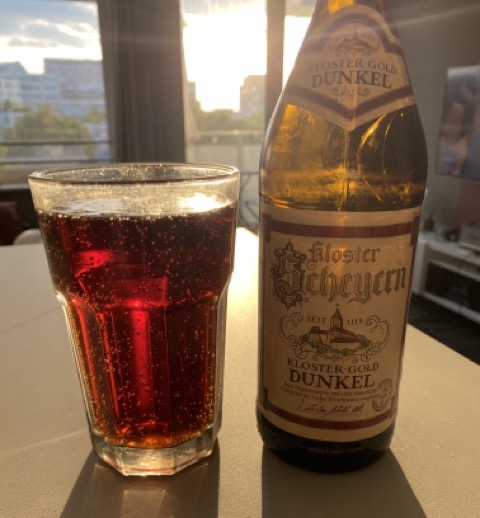
\includegraphics[height=3.2cm]{img/beer3.jpeg}}\\
    \vfill
    \onslide<+->{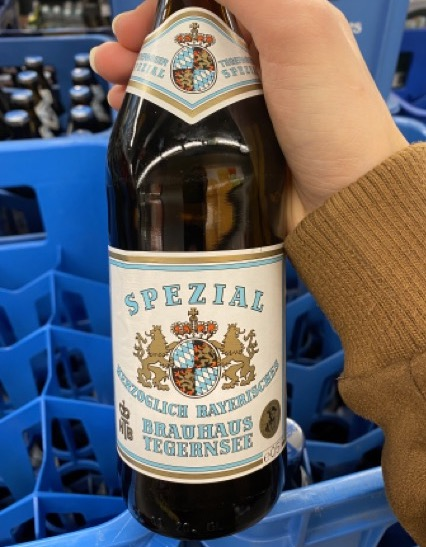
\includegraphics[height=3.2cm]{img/beer4.jpeg}}
    \onslide<+->{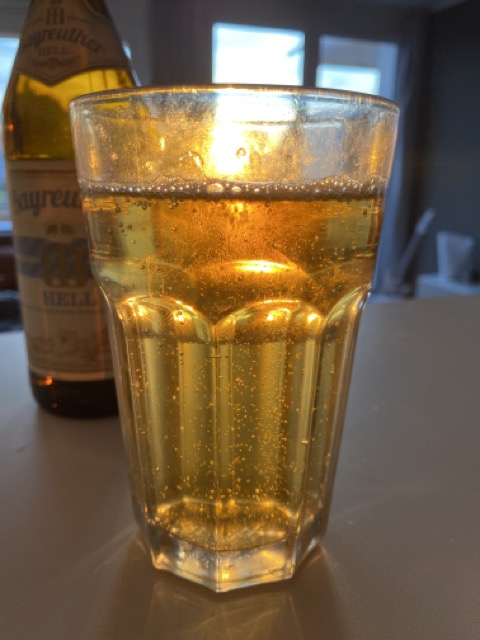
\includegraphics[height=3.2cm]{img/beer5.jpeg}}
    \onslide<+->{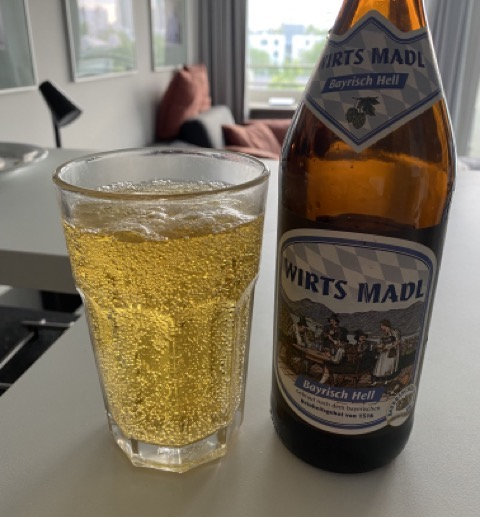
\includegraphics[height=3.2cm]{img/beer6.jpeg}}
    \onslide<+->{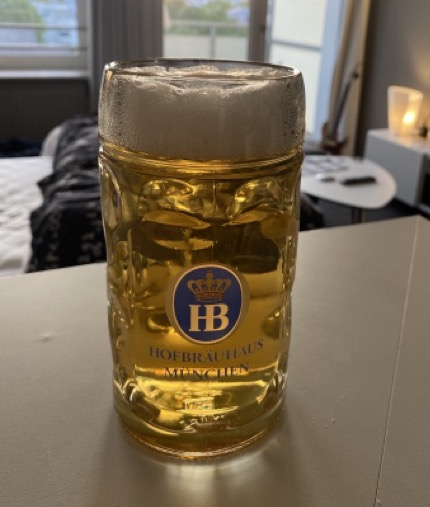
\includegraphics[height=3.2cm]{img/beer7.jpeg}}
\end{figure}
}
\end{frame}

\section{The Isabelle Refinement Framework}

\begin{frame}
    \tableofcontents[currentsection]
\end{frame}

\begin{frame}
\frametitle{Understanding Refinement}

% Spoken content:
\begin{definition}
  Refinement is a systematic process of refining a high-level abstract specification into a concrete implementation.
\end{definition}

\onslide<2->{
\begin{center}
  \begin{tikzpicture}
    \small
    \node[draw=maincolor, very thick, fill=maincolor!20, rounded corners=0.5cm, minimum width=3cm, minimum height=1cm] (spec) {Specification};
    \node[minimum height=.5cm, below of=spec, yshift=-.5cm] (aux) {\dots};
    \node[draw=orange!90!black, fill=orange!40, very thick, rounded corners=0.5cm, minimum width=3cm, minimum height=1cm, below of=aux, yshift=-.5cm] (impl) {Implementation};

    \only<2>{
    \node[minimum height=.5cm, left of=aux, xshift=-2cm] (topdown) {Top-down};

    \draw[->] (spec) -- node[right] {Refinement} (aux);
    \draw[->] (aux) -- node[right] {Refinement} (impl);
    }
    \only<3>{
    \node[minimum height=.5cm, left of=aux, xshift=-2cm] (topdown) {Bottom-up};

    \draw[->] (impl) -- node[right] {Abstraction} (aux);
    \draw[->] (aux) -- node[right] {Abstraction} (spec);
    }
  \end{tikzpicture}
\end{center}
}
\end{frame}

\begin{frame}
  Each refinement step preserves the intended behavior.

  $$\texttt{Spec} \rightarrow \texttt{Ref}_1 \rightarrow \texttt{Ref}_2 \rightarrow \texttt{Impl}$$

  \begin{center}
  \begin{tikzpicture}
    \small
    \node[ellipse, thick, draw=none, fill=maincolor!20, minimum width=5cm, minimum height=4cm] (spec) at (0,0) {}; 
    \node[yshift=-.3cm] at (spec.north) {\color{maincolor!80!black}\texttt{Spec}};

    \node[ellipse, thick, draw=none, fill=blue!15, minimum width=4cm, minimum height=3.2cm] (spec) at (-.3cm,-.1cm) {}; 
    \node[yshift=-.3cm] at (spec.north) {\color{blue!70!black}\texttt{Ref}$_1$};

    \node[ellipse, thick, draw=none, fill=purple!20, minimum width=3cm, minimum height=2.5cm] (spec) at (-.1cm,-.3cm) {}; 
    \node[yshift=-.3cm] at (spec.north) {\color{purple!70!black}\texttt{Ref}$_2$};

    \node[ellipse, thick, draw=none, fill=orange!80!black!20, minimum width=2cm, minimum height=1.5cm] (spec) at (-.1cm,-.5cm) {}; 
    \node[yshift=-.3cm] at (spec.north) {\color{orange!70!black}\texttt{Impl}};

    \node[yshift=-2cm] at (spec.south) {\Large\faThumbsOUp};
  \end{tikzpicture}
  \hfill
  \begin{tikzpicture}
    \small
    \node[ellipse, thick, draw=none, fill=orange!80!black!20, minimum width=5cm, minimum height=4cm] (spec) at (0,0) {}; 
    \node[yshift=-.3cm] at (spec.north) {\color{orange!70!black}\texttt{Impl}};

    \node[ellipse, thick, draw=none, fill=maincolor!20, minimum width=3cm, minimum height=2.5cm] (spec) at (-.1cm,-.3cm) {}; 
    \node[yshift=-.3cm] at (spec.north) {\color{maincolor}\texttt{Spec}};

    \node[yshift=-2cm] at (spec.south) {\Large\faThumbsODown};
  \end{tikzpicture}
  \end{center}
\end{frame}

\begin{frame}
  \frametitle{The Isabelle Refinement Framework}

  % Spoken content:
  % The Isabelle Refinement Framework is a powerful tool for applying refinement in a formal and mathematical way.
  % It was designed by Peter Lammich and his collaborators.

  \begin{block}{Isabelle Refinement Framework}
    \begin{itemize}
      \item Stepwise refinement approach to verified program development
      \item Formal and mathematical
      \item Ensures correctness at each step
    \end{itemize}
  \end{block}
  Comes with the Isabelle Collection Framework, which provides an extensive library of reusable verified functional data structures (for data refinement).
\end{frame}

\section{Hopcroft's algorithm}

\begin{frame}
    \tableofcontents[currentsection]
\end{frame}

\subsection{DFA minimization by example}
\begin{frame}
    \centering
    \small

    \onslide<1->{
      \only<5->{
      \setbeamercovered{transparent}
      \begin{minipage}[c]{0.55\linewidth}
        \setlength{\interspacetitleruled}{0pt}%
        \setlength{\algotitleheightrule}{0pt}%
        \SetKwIF{If}{ElseIf}{Else}{if}{}{else if}{else}{end if}%
        \begin{algorithm}[H]
          \scriptsize
          \SetInd{0.6em}{0.6em}
          \SetAlgoNoLine
          \DontPrintSemicolon
          \label{alg:modern}
          \uncover<5>{
          \KwData{a DFA $\mathcal{A} = (\mathcal{Q}, \Sigma, \delta, q_0, \mathcal{F})$}
          }
          \uncover<5>{
          \eIf{$\mathcal{F} = \varnothing \lor \mathcal{Q} \setminus \mathcal{F} = \varnothing$}{
              \Return $\mathcal{Q}$
          }}{
            \uncover<5-6>{
              $\mathcal{P} := \{ \mathcal{F}, \mathcal{Q} \setminus \mathcal{F} \}$ \;
              $\mathcal{W} := \{ (a, \min \{ \mathcal{F}, \mathcal{Q} \setminus \mathcal{F}\}), a \in \Sigma \}$ \;
            }
            \uncover<5,7->{
              \While{$\mathcal{W} \neq \varnothing$}{
                  Pick $(a, C)$ from $\mathcal{W}$ and remove it\;
                  \ForAll{$B \in \mathcal{P}$}{
                      Split $B$ with $(a, C)$ into $B_0$ and $B_1$ \;
                      $\mathcal{P} := (\mathcal{P} \setminus \{B\}) \cup \{B_0, B_1\}$ \;
                      \ForAll{$b \in \Sigma$}{
                          \eIf{$(b, B) \in \mathcal{W}$}{
                              $\mathcal{W} := (\mathcal{W} \setminus \{(b, B)\}) \cup \{(b, B_0), (b, B_1)\}$ \;
                          }{
                              $\mathcal{W} := \mathcal{W} \cup \{(b, \min \{ B_0, B_1 \})\}$ \;
                          }
                      }
                  }
              }
            }
          }
        \end{algorithm}
      \end{minipage}
      }
    \setbeamercovered{invisible}
    \begin{minipage}[c]{0.4\linewidth}
    \begin{tikzpicture}[shorten >=1pt,node distance=2cm, on grid, >={Stealth[round]},initial text=,
        every state/.style={draw=maincolor,very thick,fill=maincolor!20}]
     
        \only<1-5>{\node[state, initial] (q0) {$q_0$}};
        \only<6->{\node[state, initial, fill=orange!40, draw=orange!90!black] (q0) {$q_0$}};

        \only<1-5>{\node[state, right of=q0] (q1) {$q_1$}};
        \only<6->{\node[state, right of=q0, fill=orange!40, draw=orange!90!black] (q1) {$q_1$}};
        \only<1-5>{\node[state, accepting, below of=q0] (q2) {$q_2$}};
        \only<6->{\node[state, accepting, below of=q0, fill=blue!30, draw=blue!70] (q2) {$q_2$}};

        \only<1-5>{\node[state, accepting, below of=q1] (q3) {$q_3$}};
        \only<6->{\node[state, accepting, below of=q1, fill=blue!30, draw=blue!70] (q3) {$q_3$}};

        \only<1-5>{\node[state, accepting, below of=q2] (q4) {$q_4$}};
        \only<6->{\node[state, accepting, below of=q2, fill=blue!30, draw=blue!70] (q4) {$q_4$}};
        \only<1-5>{\node[state, below of=q3] (q5) {$q_5$}};
        \only<6-7>{\node[state, below of=q3, fill=orange!40, draw=orange!90!black] (q5) {$q_5$}};
        \only<8->{\node[state, below of=q3] (q5) {$q_5$}};

        \path[->] (q0) edge[bend left] node[above]{$\alpha$} (q1);
        \path[->] (q0) edge node[left]{$\beta$} (q2);
        \path[->] (q1) edge[bend left] node[below]{$\alpha$} (q0);
        \path[->] (q1) edge node[right]{$\beta$} (q3);
        \path[->] (q2) edge node[left]{$\alpha$} (q4);
        \path[->] (q2) edge node[left=.3cm]{$\beta$} (q5);
        \path[->] (q3) edge node[right]{$\beta$} (q5);
        \path[->] (q3) edge node[above=.3cm]{$\alpha$} (q4);
        \path[->] (q4) edge[loop below] node[below]{$\alpha$} (q4);
        \path[->] (q4) edge node[below]{$\beta$} (q5);
        \path[->] (q5) edge[loop below] node[below]{$\alpha,\beta$} (q5);
    \end{tikzpicture}
    }
    \end{minipage}

    \only<1-10>{
    \begin{table}
        \centering
        \small
        \only<1-4>{
            \begin{itemize}
                \item<2-> Successively partitions the set of states into equivalence classes
                \item<3-> Initial partition: accepting and non-accepting states
                \item<4-> Each iteration: pick a splitter and split all blocks of the current partition
            \end{itemize}
        }
        \onslide<6->{\begin{tabular}{c|c|c}
          \small
            Splitter & Partition & Workset\\
            \hline
            -- & $\{{\color{orange!80!black}q_0,q_1, q_5}\}\{{\color{blue!70}q_2, q_3, q_4}\}$ & $(\alpha, \{{\color{orange!80!black}q_0,q_1, q_5}\})\ (\beta, \{{\color{orange!80!black}q_0,q_1, q_5}\})$\\
            \onslide<8->{$(\beta, \{{\color{orange!80!black}q_0,q_1, q_5}\})$ & $\{{\color{orange!80!black}q_0,q_1}\}\{{\color{maincolor!80!black}q_5}\}\{{\color{blue!70}q_2, q_3, q_4}\}$ & $(\alpha, \{{\color{orange!80!black}q_0,q_1}\})\ (\alpha, \{{\color{maincolor!80!black}q_5}\})$}\\
            \onslide<9->{$(\alpha, \{{\color{orange!80!black}q_0,q_1}\})$ & $\{{\color{orange!80!black}q_0,q_1}\}\{{\color{maincolor!80!black}q_5}\}\{{\color{blue!70}q_2, q_3, q_4}\}$ & $(\alpha, \{{\color{maincolor!80!black}q_5}\})$}\\
            \onslide<10->{$(\alpha, \{{\color{maincolor!80!black}q_5}\})$ & $\{{\color{orange!80!black}q_0,q_1}\}\{{\color{maincolor!80!black}q_5}\}\{{\color{blue!70}q_2, q_3, q_4}\}$ & $\varnothing$}\\
        \end{tabular}}
    \end{table}
    }
\end{frame}

\begin{frame}
  \centering
  \begin{tikzpicture}[shorten >=1pt,node distance=2.3cm, on grid, >={Stealth[round]},initial text=,
    every state/.style={draw=maincolor,very thick,fill=maincolor!20}]
    \centering
    \small
    \node[state, initial, draw=orange!90!black, fill=orange!40] (Q0) {$q_0, q_1$};
    \node[state, accepting, below of=Q0, draw=blue!70, fill=blue!30] (Q1) {$q_2,q_3,q_4$};
    \node[state, below of=Q1] (Q2) {$q_5$};
    
    % Invisible for alignment
    \node[draw=none, below of=Q2, yshift=1.6cm] (Q2text) {};

    \path[->] (Q0) edge[loop right] node[right]{$\alpha$} (Q0);
    \path[->] (Q0) edge node[right]{$\beta$} (Q1);
    \path[->] (Q1) edge[loop right] node[right]{$\alpha$} (Q1);
    \path[->] (Q1) edge node[right]{$\beta$} (Q2);
    \path[->] (Q2) edge[loop right] node[right]{$\alpha,\beta$} (Q2);
\end{tikzpicture}
\begin{tikzpicture}[shorten >=1pt,node distance=2cm, on grid, >={Stealth[round]},initial text=,
  every state/.style={draw=maincolor,very thick,fill=maincolor!20}]
  \centering\small

  \node[state, initial, fill=orange!40, draw=orange!90!black] (q0) {$q_0$};

  \node[state, right of=q0, fill=orange!40, draw=orange!90!black] (q1) {$q_1$};

  \node[state, accepting, below of=q0, fill=blue!30, draw=blue!70] (q2) {$q_2$};


  \node[state, accepting, below of=q1, fill=blue!30, draw=blue!70] (q3) {$q_3$};


  \node[state, accepting, below of=q2, fill=blue!30, draw=blue!70] (q4) {$q_4$};


  \node[state, below of=q3] (q5) {$q_5$};

  \path[->] (q0) edge[bend left] node[above]{$\alpha$} (q1);
  \path[->] (q0) edge node[left]{$\beta$} (q2);
  \path[->] (q1) edge[bend left] node[below]{$\alpha$} (q0);
  \path[->] (q1) edge node[right]{$\beta$} (q3);
  \path[->] (q2) edge node[left]{$\alpha$} (q4);
  \path[->] (q2) edge node[left=.3cm]{$\beta$} (q5);
  \path[->] (q3) edge node[right]{$\beta$} (q5);
  \path[->] (q3) edge node[above=.3cm]{$\alpha$} (q4);
  \path[->] (q4) edge[loop below] node[below]{$\alpha$} (q4);
  \path[->] (q4) edge node[below]{$\beta$} (q5);
  \path[->] (q5) edge[loop below] node[below]{$\alpha,\beta$} (q5);
\end{tikzpicture}
$$\mathcal{L} = \alpha^*\beta\alpha^*$$
\end{frame}

\subsection{To be named}

\begin{frame}
    Formalization
\end{frame}

\subsection{Application to Hopcroft's algorithm}

\begin{frame}
    Coming soon
\end{frame}

\end{document}